\documentclass{article}
\usepackage{graphicx, tikz-cd, float, titlepic, booktabs} % Required for inserting images
\usepackage{pgfplots}
\usepackage{multicol}
\usepackage{makecell}
\pgfplotsset{compat=1.15}
\usepackage{mathrsfs}
\usetikzlibrary{arrows}
\usepackage{amsmath, amssymb, amsthm, amsfonts, siunitx, physics, gensymb}
\AtBeginDocument{\RenewCommandCopy\qty\SI}
\usepackage[version=4]{mhchem}
\usepackage[most,many,breakable]{tcolorbox}
\usepackage{xcolor, fancyhdr, varwidth}
\usepackage[Glenn]{fncychap}
%Options: Sonny, Lenny, Glenn, Conny, Rejne, Bjarne, Bjornstrup
\usepackage{hyperref, cleveref}
\usepackage{icomma, enumitem} %comma as decimal and continue enumerate with [resume]
\usepackage{plimsoll} %use standard state symbol with \stst
\usepackage[danish]{babel}
\renewcommand{\cellalign}{cl}
\renewcommand{\theadalign}{cl}
\renewcommand\theadfont{\bfseries}
%%%%%%%%%%%%%%%%%%%%%%%%%%%%%%
% SELF MADE COLORS
%%%%%%%%%%%%%%%%%%%%%%%%%%%%%%
\definecolor{myg}{RGB}{56, 140, 70}
\definecolor{myb}{RGB}{45, 111, 177}
\definecolor{myr}{RGB}{199, 68, 64}
\definecolor{mytheorembg}{HTML}{F2F2F9}
\definecolor{mytheoremfr}{HTML}{00007B}
\definecolor{mylenmabg}{HTML}{FFFAF8}
\definecolor{mylenmafr}{HTML}{983b0f}
\definecolor{mypropbg}{HTML}{f2fbfc}
\definecolor{mypropfr}{HTML}{191971}
\definecolor{myexamplebg}{HTML}{F2FBF8}
\definecolor{myexamplefr}{HTML}{88D6D1}
\definecolor{myexampleti}{HTML}{2A7F7F}
\definecolor{mydefinitbg}{HTML}{E5E5FF}
\definecolor{mydefinitfr}{HTML}{3F3FA3}
\definecolor{notesgreen}{RGB}{0,162,0}
\definecolor{myp}{RGB}{197, 92, 212}
\definecolor{mygr}{HTML}{2C3338}
\definecolor{myred}{RGB}{127,0,0}
\definecolor{myyellow}{RGB}{169,121,69}
\definecolor{myexercisebg}{HTML}{F2FBF8}
\definecolor{myexercisefg}{HTML}{88D6D1}
%%%%%%%%%%%%%%%%%%%%%%%%%%%%%%%%%%%%%%%%%%%%%%%%%%%%%%%%%%%%%%%%%%%%%%
% Box environments for theorems and problems
%%%%%%%%%%%%%%%%%%%%%%%%%%%%%%%%%%%%%%%%%%%%%%%%%%%%%%%%%%%%%%%%%%%%%
\setlength{\parindent}{1cm}
%================================
% Question BOX
%================================
\makeatletter
\newtcbtheorem{question}{Opgave}{enhanced,
	breakable,
	colback=white,
	colframe=myb!80!black,
	attach boxed title to top left={yshift*=-\tcboxedtitleheight},
	fonttitle=\bfseries,
	title={#2},
	boxed title size=title,
	boxed title style={%
			sharp corners,
			rounded corners=northwest,
			colback=tcbcolframe,
			boxrule=0pt,
		},
	underlay boxed title={%
			\path[fill=tcbcolframe] (title.south west)--(title.south east)
			to[out=0, in=180] ([xshift=5mm]title.east)--
			(title.center-|frame.east)
			[rounded corners=\kvtcb@arc] |-
			(frame.north) -| cycle;
		},
	#1
}{def}
\makeatother
%================================
% DEFINITION BOX
%================================

\newtcbtheorem[]{Definition}{Definition}{enhanced,
	before skip=2mm,after skip=2mm, colback=red!5,colframe=red!80!black,boxrule=0.5mm,
	attach boxed title to top left={xshift=1cm,yshift*=1mm-\tcboxedtitleheight}, varwidth boxed title*=-3cm,
	boxed title style={frame code={
					\path[fill=tcbcolback]
					([yshift=-1mm,xshift=-1mm]frame.north west)
					arc[start angle=0,end angle=180,radius=1mm]
					([yshift=-1mm,xshift=1mm]frame.north east)
					arc[start angle=180,end angle=0,radius=1mm];
					\path[left color=tcbcolback!60!black,right color=tcbcolback!60!black,
						middle color=tcbcolback!80!black]
					([xshift=-2mm]frame.north west) -- ([xshift=2mm]frame.north east)
					[rounded corners=1mm]-- ([xshift=1mm,yshift=-1mm]frame.north east)
					-- (frame.south east) -- (frame.south west)
					-- ([xshift=-1mm,yshift=-1mm]frame.north west)
					[sharp corners]-- cycle;
				},interior engine=empty,
		},
	fonttitle=\bfseries,
	title={#2},#1}{def}
\newtcbtheorem[]{definition}{Definition}{enhanced,
	before skip=2mm,after skip=2mm, colback=red!5,colframe=red!80!black,boxrule=0.5mm,
	attach boxed title to top left={xshift=1cm,yshift*=1mm-\tcboxedtitleheight}, varwidth boxed title*=-3cm,
	boxed title style={frame code={
					\path[fill=tcbcolback]
					([yshift=-1mm,xshift=-1mm]frame.north west)
					arc[start angle=0,end angle=180,radius=1mm]
					([yshift=-1mm,xshift=1mm]frame.north east)
					arc[start angle=180,end angle=0,radius=1mm];
					\path[left color=tcbcolback!60!black,right color=tcbcolback!60!black,
						middle color=tcbcolback!80!black]
					([xshift=-2mm]frame.north west) -- ([xshift=2mm]frame.north east)
					[rounded corners=1mm]-- ([xshift=1mm,yshift=-1mm]frame.north east)
					-- (frame.south east) -- (frame.south west)
					-- ([xshift=-1mm,yshift=-1mm]frame.north west)
					[sharp corners]-- cycle;
				},interior engine=empty,
		},
	fonttitle=\bfseries,
	title={#2},#1}{def}

\newtcbtheorem{theo}%
    {Theorem}{}{theorem}
\newtcolorbox{prob}[1]{colback=red!5!white,colframe=red!50!black,fonttitle=\bfseries,title={#1}}
%================================
% NOTE BOX
%================================

\usetikzlibrary{arrows,calc,shadows.blur}
\tcbuselibrary{skins}
\newtcolorbox{note}[1][]{%
	enhanced jigsaw,
	colback=gray!20!white,%
	colframe=gray!80!black,
	size=small,
	boxrule=1pt,
	title=\textbf{Note:},
	halign title=flush center,
	coltitle=black,
	breakable,
	drop shadow=black!50!white,
	attach boxed title to top left={xshift=1cm,yshift=-\tcboxedtitleheight/2,yshifttext=-\tcboxedtitleheight/2},
	minipage boxed title=1.5cm,
	boxed title style={%
			colback=white,
			size=fbox,
			boxrule=1pt,
			boxsep=2pt,
			underlay={%
					\coordinate (dotA) at ($(interior.west) + (-0.5pt,0)$);
					\coordinate (dotB) at ($(interior.east) + (0.5pt,0)$);
					\begin{scope}
						\clip (interior.north west) rectangle ([xshift=3ex]interior.east);
						\filldraw [white, blur shadow={shadow opacity=60, shadow yshift=-.75ex}, rounded corners=2pt] (interior.north west) rectangle (interior.south east);
					\end{scope}
					\begin{scope}[gray!80!black]
						\fill (dotA) circle (2pt);
						\fill (dotB) circle (2pt);
					\end{scope}
				},
		},
	#1,
}
%================================
% EXAMPLE BOX
%================================
\newtcbtheorem[number within=section]{Example}{Example}
{%
	colback = myexamplebg
	,breakable
	,colframe = myexamplefr
	,coltitle = myexampleti
	,boxrule = 1pt
	,sharp corners
	,detach title
	,before upper=\tcbtitle\par\smallskip
	,fonttitle = \bfseries
	,description font = \mdseries
	,separator sign none
	,description delimiters parenthesis
}
{ex}
%================================
% THEOREM BOX
%================================

\tcbuselibrary{theorems,skins,hooks}
\newtcbtheorem[number within=section]{Theorem}{Theorem}
{%
	enhanced,
	breakable,
	colback = mytheorembg,
	frame hidden,
	boxrule = 0sp,
	borderline west = {2pt}{0pt}{mytheoremfr},
	sharp corners,
	detach title,
	before upper = \tcbtitle\par\smallskip,
	coltitle = mytheoremfr,
	fonttitle = \bfseries\sffamily,
	description font = \mdseries,
	separator sign none,
	segmentation style={solid, mytheoremfr},
}
{th}

%%%%%%%%%%%%%%%%%%%%%%%%%%%%%%%%%%%%%%%%%%%%%%%%%%%%%%%%%%%%%%%%%
% SELF MADE COMMANDS
%%%%%%%%%%%%%%%%%%%%%%%%%%%%%%
\newcommand{\sol}{\setlength{\parindent}{0cm}\textbf{\textit{Løsning:}}\setlength{\parindent}{1cm}}
%%%%%%%%%%%%%%%%%%%%%%%%%%%%%%%%%
\usepackage[tmargin=2cm,rmargin=1in,lmargin=1in,margin=0.85in,bmargin=2cm,footskip=.2in]{geometry}\pagestyle{fancy}
\lhead{Minrui Kevin Zhou 3.b}
\rhead{Aflevering 39}

\title{Aflevering 39\\
{\Large \textbf{3.b mat A}}}
\author{Kevin Zhou}
\date{\today}

\begin{document}
\maketitle
\newpage
\begin{question}{Opgave 10: Model for udvikling af fiskebestand}{}
  En fiskeribiolog undersøger udviklingen i antallet af fisk i et stort bassin.
Udviklingen kan beskrives ved differentialligningen
\[
  y'=0,5 \cdot y \cdot \left(1-0,0002 \cdot y\right) -0,06 \cdot y
\] 
hvor $y$ er antallet af fisk i bassinet $t$ år efter undersøgelsens start.
Ved undersøgelsens start er der 3500 fisk i bassinet. 
\end{question}
\sol \\
\textbf{a.}
For at finde hastigheden af fiskeudviklingen ved undersøgelsens start, ved at sætte $y=3500$ ind i ligningen. 
Når $y=3500$ gælder der 
\begin{equation*}
\begin{split}
  y'&=0,5 \cdot 3500 \cdot \left(1-0,0002 \cdot 3500\right) -0,06 \cdot 3500\\
  &=315
\end{split}
\end{equation*}
Ved undersøgelsens start vokser antallet af fisk i bassinet altså med hastigheden 315 fisk per år.\\[1ex]
\textbf{b.}
For at bestemme antallet af fisk efter fem år, findes en forskrift for løsningen af differentialligningen, som vi betegner $f$.
Vi omskriver først udtrykket for $y'$.
\begin{equation*}
\begin{split}
  y'=0,5 \cdot y \cdot \left(1-0,0002 \cdot y\right) -0,06 \cdot y &\iff y'=y \cdot \left(0,5 - 0,06 - 0,0002 \cdot 0,5 \cdot y\right) \\
  &\iff y'=y \cdot \left(0,44-0,0001 \cdot y\right) 
\end{split}
\end{equation*}
Siden en differentialligning af formen $y'=y \cdot \left(b-a \cdot y\right) $ har de ikke-trivielle løsninger $y=\frac{\frac{b}{a}}{1+c \cdot e^{-bt} }$, så må $f$ være af formen 
\begin{equation*}
\begin{split}
f(t)&=\frac{\frac{0,44}{0,0001}}{1+ c \cdot e^{-0,44 \cdot t} }\\
&=\frac{4400}{1+c \cdot e^{-0,44 \cdot t} }
\end{split}
\end{equation*}
Siden $f(0)=3500$, så har vi 
\begin{equation*}
\begin{split}
  f(0)= 3500 &\iff 3500 = \frac{4400}{1+c \cdot e^{-0,44 \cdot 0} }\\
  &\iff 1+c=\frac{4400}{3500}\\
  &\iff c=\frac{9}{35}
\end{split}
\end{equation*}
Vi har altså 
\[
f(t)=\frac{4400}{1+\frac{9}{35}\cdot e^{-0,44 \cdot t} }
\] 
Vi beregner nu $f(5)$.
\begin{equation*}
\begin{split}
  f(5)&=\frac{4400}{1+\frac{9}{35}\cdot e^{-0,44 \cdot 5} }\\
  &\approx 4278
\end{split}
\end{equation*}
Antallet af fisk i bassinet efter 5 år er altså 4278.
\begin{question}{Opgave 11: Arealbestemmelse}{}
  Funktionen $f$ er givet ved
  \[
  f(x)= 2x-\frac{1}{2}x^3
  \] 
Grafen for $f$ afgrænser sammen med førsteaksen i første kvadrant et område $M$.
  I \cref{fig:f} ses først grafen for $f$ og så grafen for $f$ med en lodret linje med ligning $x=k$, hvor $0<k<2$, som deler $M$ i to dele.
\end{question}
\begin{figure}[H]
\begin{center}
  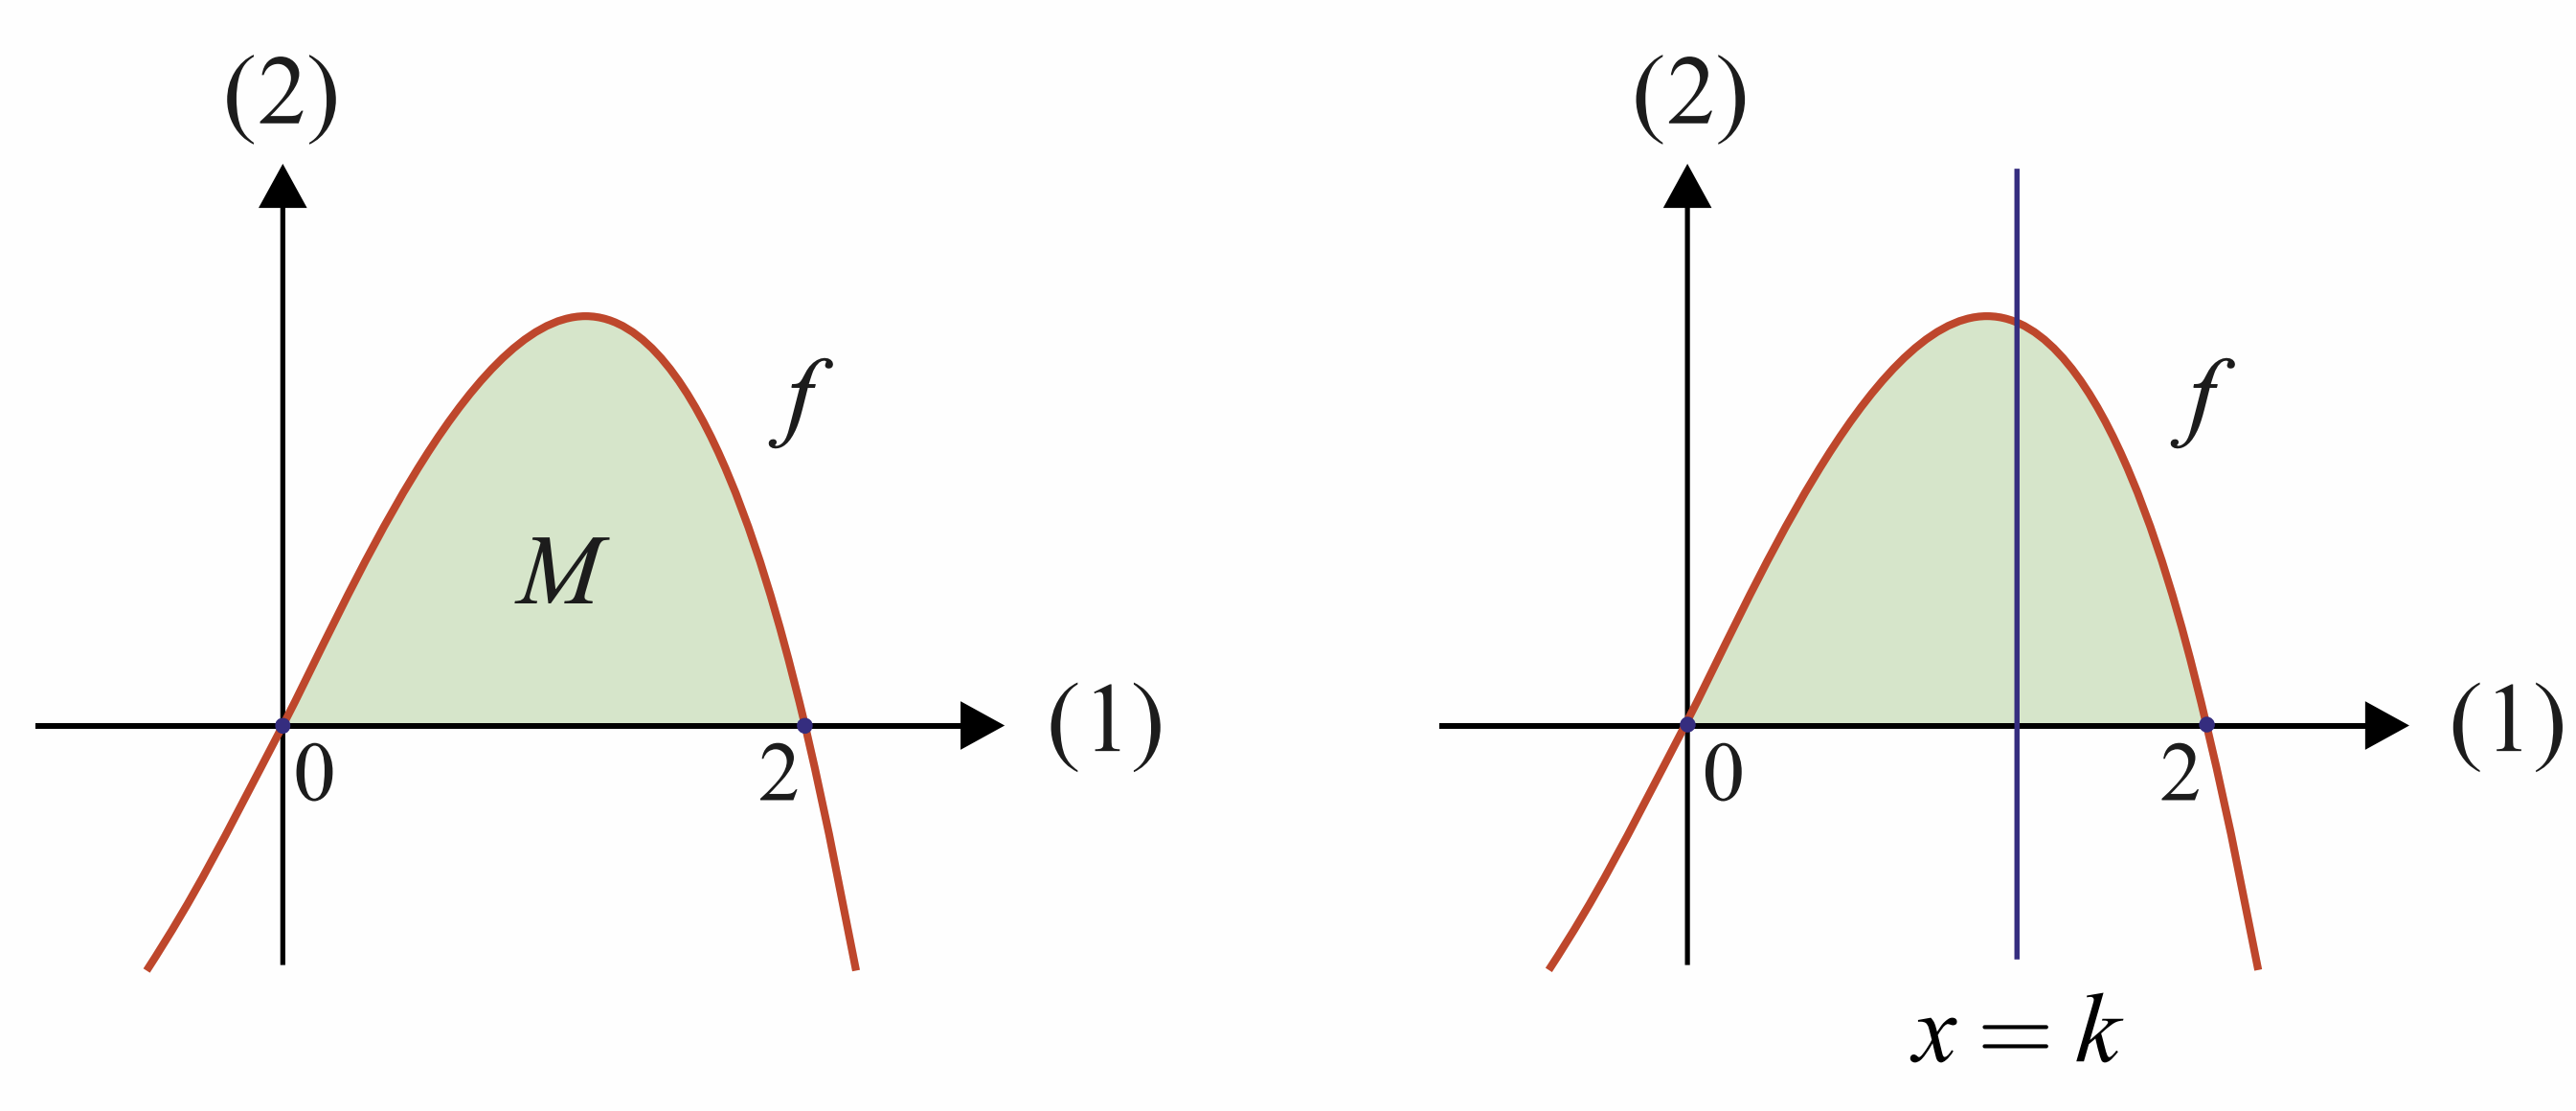
\includegraphics[width=\textwidth]{f.png}
\end{center}
  \caption{Grafen for $f$ og lodret linje med ligningen $x=k, \quad 0<k<2$}
\label{fig:f}
\end{figure}
\sol \\
\textbf{a.}
Vi ser fra \cref{fig:f}, at grafen for $f$ skærer førsteaksen ved $x=0$ og $x=2$. 
Siden der gælder, at $x \in [0;2] \implies f(x) \geq 0$, så må arealet af $M$ være
\begin{equation*}
\begin{split}
  A(M)&=\int_{0}^{2} f(x) \,dx \\
  &=\int_{0}^{2} \left(2x - \frac{1}{2}x^3\right)  \,dx \\
  &=\left[x^2-\frac{1}{8}x^4\right]_0^2\\
  &=2^2-\frac{2^4}{2^3}\\
  &=4-2\\
  &=2
\end{split}
\end{equation*}
Arealet af $M$ er altså 2.\\[1ex]
\textbf{b.}
Vi vil gerne finde $k$, når de to områder har samme areal. 
De to områder har samme areal netop når (bemærk at $k>0$)
\begin{equation*}
\begin{split}
  \int_{0}^{k} f(x) \,dx = \int_{k}^{2} f(x) \,dx &\iff \left[x^2-\frac{1}{8}x^4\right]_0^k=\left[x^2-\frac{1}{8}x^4\right]_k^2\\
  &\iff 2 \cdot \left(k^2-\frac{1}{8}k^4\right) =2^2-\frac{1}{8}\cdot 2^4\\
  &\iff k^2-\frac{1}{8}k^4=1\\
  &\iff -\frac{1}{8}k^4+k^2-1=0\\
  &\iff k^2=\frac{-1 - \sqrt{1^2-4 \cdot \left(-\frac{1}{8} \right) \cdot \left(-1\right) } }{2 \cdot \left(-\frac{1}{8}\right) }\\
  &\iff k^2=-4 \cdot \left(-1 - \sqrt{\frac{1}{2}} \right) \\
  &\iff k=\sqrt{4+4 \cdot \sqrt{\frac{1}{2}} } \\
  &\iff k=\sqrt{4+2 \sqrt{2} }
\end{split}
\end{equation*}
Bemærk, at grunden til, at vi kun får 1 løsning er, at vi benytter det faktum, at $k$ er positiv.
De to dele af området får altså samme areal når $k=\sqrt{4+2 \sqrt{2} } $.
\begin{question}{Opgave 13: Logo for TV-station og vekterfunktion}{}
  Logoet for TV-stationen Australian Broadcasting Corporation har form som
parameterkurven for vektorfunktionen $\vec{r}$ givet ved

$$\vec{r}\left(t\right)=\binom{\cos(t)}{\sin(3t)},\quad0\leq t\leq2\pi.$$
  Parameterkurven for $\va{r} $ har et dobbeltpunkt for $t=\frac{\pi }{3}$ og $t=\frac{5 \pi }{3}$. 
\end{question}
\sol \\
\textbf{a.}
Parameterkurven for $\va{r} $ ses tegnet i GeoGebra i \cref{fig:param}.
\begin{figure}[H]
\begin{center}
  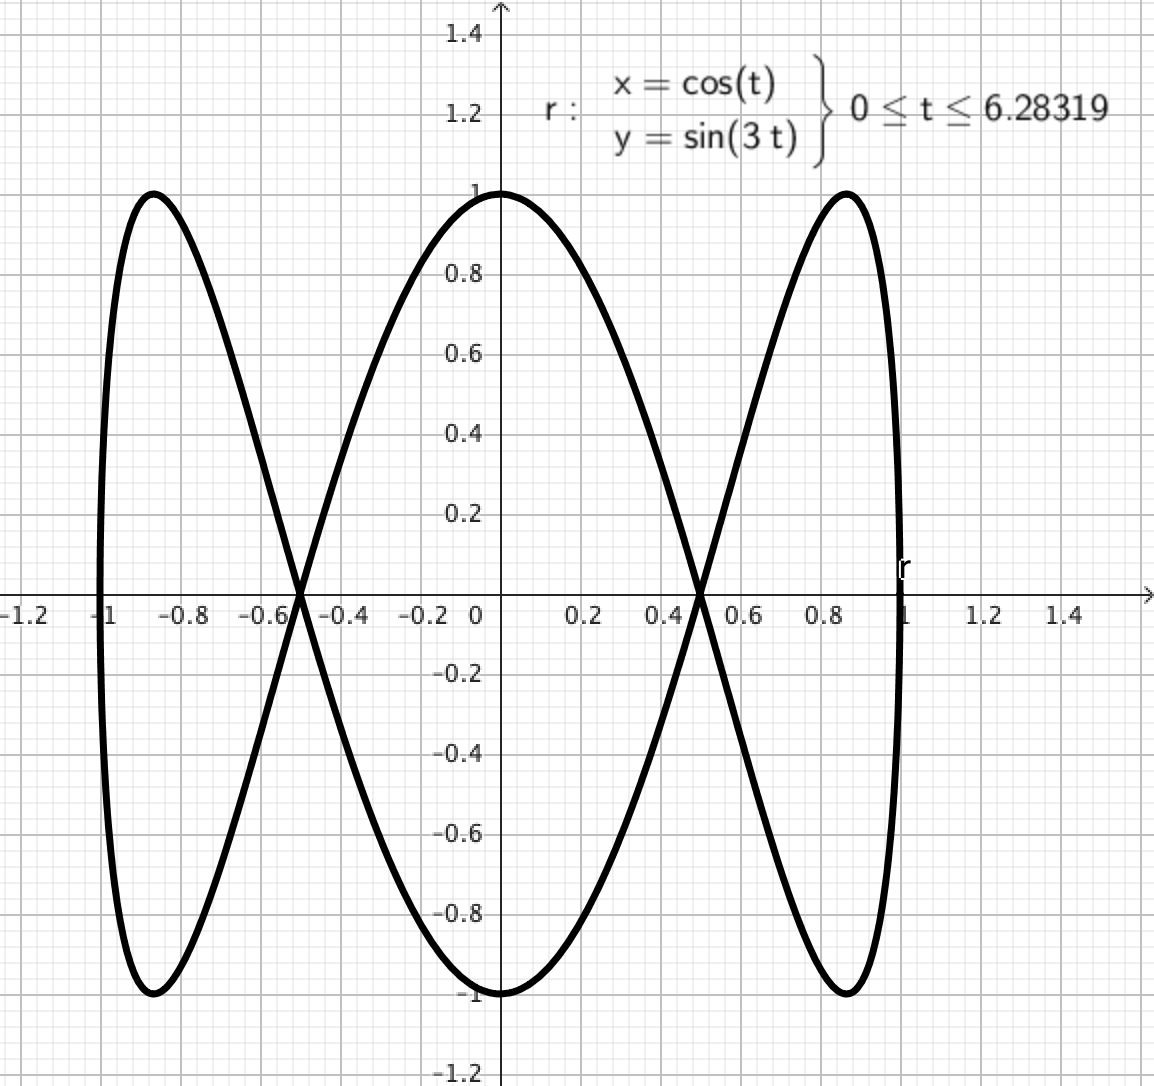
\includegraphics[width=0.7\textwidth]{parameter.png}
\end{center}
\caption{Parameterkurven for $\va{r} $ tegnet i GeoGebra }
\label{fig:param}
\end{figure}
\textbf{b.}
For at bestemme koordinatsættene til parameterkurvens skæringspunkter med andenaksen findes de tilsvarende $t$-værdier først.
Når parameterkurven skærer $y$-aksen er $x$-værdien $0$, hvilket er tilfældet når 
\begin{equation*}
\begin{split}
  \cos\left(t\right) =0 \land 0 \leq t \leq 2 \pi \implies t=\frac{1}{2}\pi \lor t=\frac{3}{2} \pi 
\end{split}
\end{equation*}
Vi beregner nu stedvektoren til de to skæringspunkter med andenaksen.
\begin{equation*}
\begin{split}
  \va{r} \left( \frac{1}{2}\pi \right)&=\mqty(0\\ \sin\left(3 \cdot \frac{1}{2} \pi \right) ) =\mqty(0\\ -1) \\
  \va{r} \left(\frac{3}{2} \pi \right) &=\mqty(0\\ \sin\left(3 \cdot \frac{3}{2} \pi  \right) ) =\mqty(0\\ 1) 
\end{split}
\end{equation*}
Koordinatsættene til parameterkurvens skæringspunkter med andenaksen er altå $(0,-1)$ og $(0,1)$.\\[1ex]
\textbf{c.}
For at finde vinklen mellem hastighedsvektorerne i dobbeltpunktet findes først et generelt udtryk for hastighedsvektorens udtrykt ved $t$, som vi betegner $\va{v}(t)$.
\begin{equation*}
\begin{split}
  \va{v}(t)&=\va{r}'(t)\\
  &=\mqty(\dv{t}\cos\left(t\right)  \\ \dv{t} \sin\left(3t\right))  \\
  &=\mqty(-\sin\left(t\right) \\ 3 \cdot \cos\left(3t\right) ) 
\end{split}
\end{equation*}
De to hastighedsvektorer i dobbeltpunktet må da være
\begin{equation*}
\begin{split}
  \va{v} \left(\frac{\pi }{3}\right) &=\mqty(-\sin\left(\frac{\pi }{3}\right) \\ 3 \cdot \cos\left(3 \cdot \frac{\pi }{3}\right) ) =\mqty(-\frac{\sqrt{3} }{2}\\ -3) \\
  \va{v} \left(\frac{5 \pi }{3}\right) &=\mqty(-\sin\left(\frac{5 \pi }{3}\right) \\ 3 \cdot \cos\left(3 \cdot \frac{5 \pi }{3}\right) ) =\mqty(\frac{\sqrt{3} }{2}\\ -3) 
\end{split}
\end{equation*}
Vi kan nu beregne vinklen mellem de to vektorer
\begin{equation*}
\begin{split}
  v&=\cos^{-1}\left(\frac{\mqty(-\frac{\sqrt{3} }{2}\\ -3) \cdot \mqty(\frac{\sqrt{3} }{2}\\ -3) }{\abs{\mqty(-\frac{\sqrt{3} }{2}\\ -3)} \cdot \abs{\mqty(\frac{\sqrt{3} }{2}\\ -3)}}\right) \\
  &=\cos^{-1}\left( \frac{-\frac{3}{4}+9}{\sqrt{\left(-\frac{\sqrt{3} }{2}\right)^2+\left(-3\right)^2} \cdot \sqrt{\left(\frac{\sqrt{3} }{2}\right)^2 + \left(-3\right)^2} }\right)\\
  &=\cos^{-1}\left(\frac{\frac{33}{4}}{\frac{3}{4}+9}\right) \\
  &=\cos^{-1}\left(\frac{33}{39}\right) \\
  &=\cos^{-1}\left(\frac{11}{13}\right) \\
  &\approx 32,204 \degree 
\end{split}
\end{equation*}
Vinklen mellem hastighedsvektorerne i dobbeltpunktet er altså $\cos^{-1}\left(\frac{11}{13}\right) \approx 32,204 \degree $.
\begin{question}{Opgave 15: Lampeskærm og funktion af to variable}{}
  \cref{fig:skærm} viser en model af en stor lampeskærm i et tredimensionalt koordinatsystem med enheden meter. I modellen kan lampeskærmen beskrives som grafen for funktionen $f:\{(x,y)\in \mathbb{R}^2 : -1 \leq x \leq 1, -1 \leq y \leq 1\} \to \mathbb{R}$ givet ved 
   \[
   f(x,y)= e^{-x^2-y^2} 
   \] 
   Punkterne $A=(1,-1,f(1,-1))$ og $B=(1,1,f(1,1))$ ligger på en af lampeskærmens kanter. 
Den ene af lampeskærmens kanter svarer til den del af snitkurven, der går fra punktet $A$ til punktet $B$. 
\end{question}
\begin{figure}[H]
\begin{center}
  \includegraphics[width=\textwidth]{skærm.png}
\end{center}
\caption{Grafen for $f$ med punkterne $A$ og $B$ }
\label{fig:skærm}
\end{figure}

\sol \\
\textbf{a.}
For at bestemme koordinatsættene for $A$ og $B$, beregner vi først deres $z$-værdier. 
\begin{equation*}
\begin{split}
  f(1,-1)&= e^{-1^2-\left(-1\right)^2} =e^{-2}\\
  f(1,1)&=e^{-1^2-1^2} = e^{-2} 
\end{split}
\end{equation*}
Vi har altså $A=(1,-1,e^{-2})$ og $B=(1,1,e^{-2})$.\\[1ex]
\textbf{b.}
For at bestemme længden af lampeskærmens kant fra $A$ til $B$, finder vi først et udtryk af den del af snitkurven, der går fra $A$ til $B$. 
Denne må da være, hvor $x=1$ (bemærk at der er tale om "kanten" pga. definitionsmængden), og vi betegner den $g$:
\begin{equation*}
\begin{split}
  g(y)&=f(1,y)\\
  &=e^{-1^2-y^2} \\
  &=e^{-1-y^2} 
\end{split}
\end{equation*}
Fra punkternes $y$-værdier er det klart, at længden af lampeskærmens kant må være kurvelængden af grafen for snitkurven fra $y=-1$ til $y=1$.
\begin{equation*}
\begin{split}
  L&=\int_{-1}^{1} \sqrt{1+g'(y)^2}  \,dy \\
  &=\int_{-1}^{1} \sqrt{1+ \left(-2y \cdot e^{-1-y^2} \right)^2}  \,dy \\
  &\approx 2,06
\end{split}
\end{equation*}
Integralet er udregnet med CAS (se \cref{fig:CAS}).
Længden af lampeskærmens kant fra punktet $A$ til $B$ er altså $2,06$ meter. 
\begin{figure}[H]
\begin{center}
  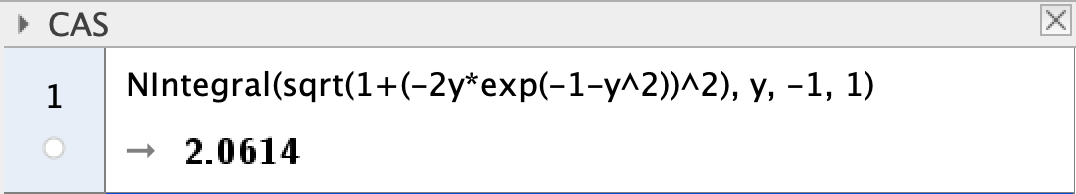
\includegraphics[width=\textwidth]{CAS.png}
\end{center}
\caption{Integralet regnet med CAS}
\label{fig:CAS}
\end{figure}





\end{document}
